{\documentclass[authoryear]{elsarticle}

\pagenumbering{gobble}


\makeatletter
\def\ps@pprintTitle{%
\let\@oddhead\@empty
\let\@evenhead\@empty
\def\@oddfoot{}%
\let\@evenfoot\@oddfoot}
\makeatother


\setlength\arraycolsep{2pt}
\setlength{\parskip}{1ex plus 0.5ex minus 0.2ex}
\usepackage{graphicx}
\usepackage{amsfonts}
\usepackage{multirow}
\usepackage{comment}

%\usepackage{chicago}
\bibliographystyle{chicago}





\newcommand{\tr}{\mathrm{tr}}
\newcommand{\e}{\mathrm{e}}
\newcommand{\de}{\mathrm{d}}






%\renewcommand{\labelenumi}{(\roman{enumi})}

\newcommand{\cq}{,\quad }
\newcommand{\qq}{\quad \Rightarrow \quad}

%REFERENCES
\newcommand{\eref}[1]{(\ref{#1})}
\newcommand{\fref}[1]{Figure \ref{#1}}
\newcommand{\sref}[1]{\S\ref{#1}}
\newcommand{\tref}[1]{Table \ref{#1}}
\newcommand{\aref}[1]{\ref{#1}}


%notation for this paper

%EXPECTATIONS AND VARIANCES
\newcommand{\var}{{\rm var}}
\newcommand{\cov}{{\rm cov}}
\newcommand{\cor}{\mathrm{cor}}
\newcommand{\E}{{\mathrm E}}
\newcommand{\p}{{\mathrm P}}
\newcommand{\Ex}{{\mathcal E}}

%DENSITIES
\newcommand{\ft}{{\tilde{f}}}
\newcommand{\Ft}{{\tilde{F}}}




\newcommand{\bi}{\begin{itemize}}
\renewcommand{\i}{\item}
\newcommand{\ei}{\end{itemize}}



\begin{document}


\begin{frontmatter}

\title{Insights to systematic risk and diversification across a joint probability distribution}




\begin{abstract}
This paper analyses and develops insights to systematic risk and diversification when random, imperfectly dependent, losses are aggregated. Systematic risk and diversification are shown to vary across layers of component losses according to local dependence and volatility structures. Systematic risk is high and diversification is weak overall if high risk layers are heavily dependent on the aggregate loss. This result explains weak diversification observed in financial markets despite weak to moderate correlations overall. A coherent risk setup is assumed in this paper, where risks are measured using distortion and allocated using the Euler principle.

\end{abstract}

\begin{keyword}
Distortion risk; spectral risk; Euler allocation; systematic risk; diversification; layer; Value--at--Risk.
\end{keyword}



\end{frontmatter}





\section{Introduction to systematic risk and diversification}\label{ssystematic}


Suppose $x$ is one of several continuous, non-negative and random component losses aggregating to $x_+$. For example $x$ may be the loss from an insurance class and $x_+$ is the loss aggregated across all classes. Or $x$ may be the credit loss on a portfolio of loans and $x_+$ is the aggregate credit loss across all portfolios. Component losses are imperfectly dependent leading to risk diversification as formalised below.


This paper applies the following risk setup. Suppose $\phi\geq 0$ is an increasing risk aversion function integrating to $1$. Standalone risk of $x$, systematic risk of $x$ and aggregate risk of $x_+$ are respectively
\begin{equation}\label{allocation}
r=\cov\{x,\phi(u)\} \cq \overline{r}=\cov\{x,\phi(u_+)\}
\cq r_+=\cov\{x_+,\phi(u_+)\}\;,
\end{equation}
where $\cov$ denotes covariance and $u$ and $u_+$ are percentile ranks of $x$ and $x_+$. If $F$ and $F_+$ are distribution functions of $x$ and $x_+$ then $u\equiv F(x)$ and $u\equiv F_+(x_+)$. Standalone and systematic risks of other component losses forming $x_+$ are calculated using similar covariance expressions.


The risk setup \eref{allocation} is well established in the literature. \cite{choo2009loss} refers to $r$ and $r_+$ as loss aversion risks of $x$ and $x_+$ and establishes their equivalence with distortion risks \citep{wang1996pct} and spectral risks \citep{acerbi2002spectral}. Examples of $\phi$ leading to different risk measures are discussed in \cite{choo2009loss}. In addition $\overline{r}$ is an allocation of $r_+$ to $x$ by applying the Euler principle \citep{mcneil2005qrm} or game theory \citep{tasche2007capital}. The allocation is extensively discussed in \cite{choo2010determining}, \cite{buch2008coherent} and \cite{tsanakas2006risk}.

The risk setup \eref{allocation} is coherent in the sense of \cite{artzner1999cmr}, \cite{denault2001coherent} and \cite{kalkbrener2005aac}: positively homogenous, translation invariant, monotonic and subadditive. Further the allocation is complete: adding $\overline{r}$ across component losses yields $r_+$, and there is no undercut: $\overline{r}\leq r$ no matter how $x$ is carved out from $x_+$.


The term ''systematic risk" is consistent with the capital asset pricing model in finance \citep{luenberger1998is}, where the volatility or risk of an asset return is divided into diversifiable and non-diversifiable or systematic risk. Systematic risk increases with the correlation between asset and market returns, and is a key driver of risk premiums: expected asset returns above market return.

This paper compares $r$, the risk of $x$ before aggregation, with $\overline{r}$, the risk of $x$ after aggregation. Since $x$ and $u_+$ are imperfectly dependent, $\overline{r} \leq r$ and the difference $r-\overline{r}$ is a diversification benefit. Diversification benefits are critical in risk management by enabling risks to be managed viably and efficiently as a group, a classic case being insurance. The systematic risk ratio is
\begin{equation}\label{ratio}
\theta \equiv \frac{\overline{r}}{r}  = \frac{\cov\{x,\phi(u_+)\} }{\cov\{x,\phi(u)\} }
=\frac{\cor\{x,\phi(u_+)\} }{\cor\{x,\phi(u)\} } \leq 1 \;,
\end{equation}
where $\cor$ represents correlation. A lower systematic risk ratio indicates greater diversification. The final expression holds since $u$ and $u_+$ are both uniform hence $\phi(u)$ and $\phi(u_+)$ have equal standard deviations. Stronger dependence between $x$ and $x_+$ leads to weaker diversification due to higher numerators in \eref{ratio} hence larger $\theta$. Conversely weaker dependence leads to stronger diversification.


In this paper, systematic risk and diversification benefit are shown to vary across the distribution of $x$ based on the local dependence structure underlying $x$ and $x_+$. This result is important when formulating risk management strategies to maximise diversification, as demonstrated by a case study using historical stock returns. The analysis focusses on $x$, however equivalent results apply to other component losses forming $x_+$.


The remaining paper is structured as follows. Section \aref{ssetup} gives an overview of mean and risk densities and Value--at--Risk (VaR) loss layers established in the second paper of this thesis (chapter 3). Section \aref{sdensity} defines systematic risk densities analogous to standalone risk densities, and establishes links to local dependence structures underlying component and aggregate losses. Section \aref{sdecompose} uses systematic risk densities to explore drivers of systematic risk and diversification such as in financial markets. A theoretical example of the proposed analytical framework is shown in \sref{segratio}. Section \aref{ssub} attributes aggregate mean and risk densities to component losses. The attribution is important when risk management strategies target the aggregate loss. Section \aref{scomono} examines the case where component losses are comonotonic, a benchmark for measuring diversification. Section \aref{seg} concludes with an illustration of the framework using historical stock returns.




\section{Overview of VaR layers, mean and risk densities}\label{ssetup}



This section outlines VaR layers, mean and risk densities developed in chapter 3 of this thesis. Mean and risk densities track the mean and standalone risk of a loss across its VaR layers. Risk densities are critical to the analysis of systematic risk and diversification as shown in subsequent sections.

The $\alpha$--Value--at--Risk (VaR$_\alpha$) of a continuous random loss $x\geq 0$ with distribution function $F$ is the percentile $V_\alpha\equiv F^-(\alpha)$, where $F^-$ is the inverse distribution function of $x$. In addition define $L_\alpha\equiv \min(x,V_\alpha)$, the loss capped at its VaR$_\alpha$. Consider the following two expressions:
$$
L_\beta-L_\alpha= \min\{\max(x-V_\alpha,0), V_\beta-V_\alpha\} \cq x=L_1-L_0=\int_0^1 \de L_\alpha \;.
$$
The first expression above is the VaR layer $[V_\alpha,V_\beta]$ of $x$: the excess of $x$ over $V_\alpha$ with the excess capped at $V_\beta-V_\alpha$. The second expression decomposes $x$ into infinitesimal VaR layers $\de L_\alpha$ over $0\le\alpha\le 1$. The infinitesimal $V_\alpha$--layer of $x$ is
$$
\de L_\alpha = L_\alpha'\de\alpha = I_\alpha(u) V_\alpha'\de \alpha   \;,
$$
where $L_\alpha'$ and $V_\alpha'$ are derivatives of $L_\alpha$ and $V_\alpha$ with respect to $\alpha$, and $I_\alpha(u)$ is an indicator equal to $1$ if $u>\alpha$ or equivalently $x>V_\alpha$, and $0$ otherwise. Hence the $V_\alpha$--layer of $x$ is an increment proportional to $V_\alpha'$ if $x>V_\alpha$ and 0 otherwise.

Layers are standard insurance and financial constructs, and are also called tranches in finance. VaR layers self-adjust to the shape and scale of the loss distribution and are hence comparable across loss distributions. Refer to chapter 3 for further discussion of layers and reasons for defining layers using VaRs.

The risk density indicates the standalone risk of infinitesimal VaR layers of $x$, and based on \eref{allocation} is the covariance
$$
r_\alpha =\cov\{L_\alpha',\phi(u)\} =\cov\{I_\alpha(u)V_\alpha',\phi(u)\} = \{\alpha-\Phi(\alpha)\}V_\alpha'   \;,
$$
where
$$
\Phi(\alpha) \equiv \int_0^\alpha \phi(u)\de u
$$
cumulates $\phi$. Integrating $r_\alpha$ yields standalone risks of larger layers:
$$
\int_\alpha^\beta r_\pi \de \pi = \cov \left\{\int_\alpha^\beta L_\pi'\de \pi ,\phi(u) \right\}
= \cov\{L_\beta-L_\alpha,\phi(u)\} \;,
$$
and the entire area under $r_\alpha$ is the overall standalone risk of $x$: $\int_0^1 r_\alpha \de \alpha =r$.

The mean density indicates the mean of infinitesimal VaR layers and is
$$
m_\alpha = \E(L_\alpha') = \E\{I_\alpha(u)V_\alpha'\} = (1-\alpha)V_\alpha' \;.
$$
Similar to $r_\alpha$, integrating $m_\alpha$ yields the mean of larger layers. Hence mean and risk densities are akin to probability densities: integrating yields quantities over larger regions. Refer to chapter 3 for further properties, illustrations and applications of mean and risk densities.






\section{Systematic risk densities and links to local dependence}\label{sdensity}


Systematic risk densities are akin to standalone risk densities in \sref{ssetup}, and describe systematic risks of infinitemisal VaR layers forming a random loss. Comparing systematic and standalone risk densities reveals the extent of diversification at various layers of the loss distribution. The comparison also leads to the dependence structure involving component and aggregate losses.


The systematic risk density of $x$ according to \eref{allocation} is the covariance
$$
\overline{r}_\alpha \equiv \cov\{L'_\alpha,\phi(u_+)\} = \cov\{I_\alpha(u),\phi(u_+)\}V_\alpha' \;.
$$
Similar to $r_\alpha$, integrating $\overline{r}_\alpha$ yields systematic risks of larger layers and the overall systematic risk of $x$:
$$
\int_\alpha^\beta \overline{r}_\pi \de \pi = \cov\left\{L_\beta-L_\alpha ,\phi(u_+)\right\}
\cq \int_0^1 \overline{r}_\alpha \de \alpha = \cov\left\{L_1 ,\phi(u_+)\right\} = \overline{r} \;.
$$
The ratio between systematic and standalone risk densities is the proportion of remaining risk in each VaR layer after diversification, and is given by
\begin{equation}\label{sysratio}
\theta_\alpha \equiv \frac{\overline{r}_\alpha}{r_\alpha}
=\frac{\cov\{I_\alpha(u)V_\alpha',\phi(u_+)\}}{\cov\{I_\alpha(u)V_\alpha',\phi(u)\}}
=\frac{\cov\{I_\alpha(u),\phi(u_+)\}}{\cov\{I_\alpha(u),\phi(u)\}} \;,
\end{equation}
where the last expression follows since the constant $V_\alpha'$ in $\overline{r}_\alpha$ and $r_\alpha$ cancel with division. If $x$ and $x_+$ are comonotonic or $u=u_+$ then $\theta_\alpha=1$ for all $0\le\alpha\le 1$. Otherwise $\theta_\alpha<1$.



For any $\alpha$, large $\theta_\alpha$ implies weak diversification at $V_\alpha$--layer of $x$ since $\overline{r}_\alpha$ is close to $r_\alpha$ and the diversification benefit $r_\alpha-\overline{r}_\alpha$ is small relative to $r_\alpha$. Vice versa diversification at $V_\alpha$--layer is strong if $\theta_\alpha$ is small or even negative. An analysis of $\theta_\alpha$ against $\alpha$ hence reveals layers with weak diversification, which can be mitigated using reinsurance or hedging, and layers with strong diversification which should be preserved since they reduce overall risk. In addition $\theta_\alpha$ varies over $\alpha$ in line with local dependence between $x$ and $x_+$. The notion is explored in the rest of this section.


The systematic risk ratio $\theta_\alpha$ is calculated entirely from the joint distribution of $(u,u_+)$ or equivalently the copula $C$ of $(x,x_+)$. Marginal distributions are not directly involved in $\theta_\alpha$, although the marginal distribution of $x$ affects $C$\footnote{For example suppose $x$ dominates other losses forming $x_+$. Then $x$ and $x_+$ are strongly dependent compared to the case where $x$ is dominated by other losses.}. The denominator of the last term in \eref{sysratio} is $\alpha-\Phi(\alpha)$ and the numerator is
$$
\int_0^1 \cov\{I_\alpha(u),I_\beta(u_+) \de \phi(\beta)=
\int_0^1 \{C(\alpha,\beta)-\alpha\beta\} \phi'(\beta) \de \beta   \;,
$$
a partial integration of the copula $C$ weighted by the derivative $\phi'$.


The set of $\theta_\alpha$ values over $0\le\alpha\le 1$ reflects and characterises the dependence structure of $(x,x_+)$. Given $\alpha$, $\theta_\alpha$ is the local dependence between $V_\alpha$--layer of $x$ and a function of the aggregate loss. Of interest is rank dependence since $\theta_\alpha$ is defined in terms of percentile ranks $u$ and $u_+$. If $(x,x_+)$ exhibits strong upper tail dependence and weak lower tail dependence, then $\theta_\alpha$ starts small at $\alpha=0$ and increases to one as $\alpha$ approaches one. An illustration of $\theta_\alpha$ given a particular $\phi$ is shown in \sref{segratio}.


Systematic risk ratios have similar properties as linear and Spearman's correlation which are measures of overall dependence. For all $0\le\alpha\le 1$, $\theta_\alpha\le 1$, $\theta_\alpha=1$ if $u=u_+$ and $\theta_\alpha=0$ if $u$ and $u_+$ are independent. Negative dependence yields $\theta_\alpha \le 0$, and $u_+=1-u$ leads to $\theta_\alpha=-1$ if $\phi(u)$ is symmetric about $u=0.5$ such that $\phi(u-0.5)=\phi(0.5-u)$. In addition stronger correlation order \citep{dhaene2009correlation} between $x$ and $x_+$ increases $\theta_\alpha$ for all $\alpha$. Proofs are straightforward from \eref{sysratio}.


Systematic risk ratios are similar to layer dependence (discussed in chapter 2 of this thesis) which measures local dependence between arbitrary uniform random variables $u$ and $v$:
$$
\ell_\alpha \equiv \frac{\cov\{I_\alpha(u),v\}}{\cov\{I_\alpha(u),u\}} \;.
$$
Layer dependence $\ell_\alpha$ assumes a linear $\phi$ in systematic risk ratio $\theta_\alpha$.





\section{Explaining and exploring systematic risk and diversification}\label{sdecompose}


High overall systematic risk ratio in \eref{ratio}, or low overall diversification, arises when strong local dependence coincides with high local skewness or volatility, such as in financial markets. High systematic risk or low diversification overall may arise even when overall correlation is weak to moderate. These intuitive concepts are formalised and explored below.



Noting $\overline{r}_\alpha=\theta_\alpha r_\alpha$ from \eref{sysratio}, overall systematic risk and risk ratio of $x$ defined in \eref{allocation} and \eref{ratio} are respectively written as
\begin{equation}\label{analysis}
\overline{r} = \int_0^1 r_\alpha \theta_\alpha \de \alpha
\cq \theta = \frac{\overline{r}}{r} = \frac{\int_0^1 r_\alpha \theta_\alpha \de \alpha }{\int_0^1 r_\alpha  \de \alpha}  \;.
\end{equation}
Similar expressions apply when considering sytematic risk over $[V_\alpha,V_\beta]$ VaR--layer of $x$: change integration limits in \eref{analysis} from $[0,1]$ to $[\alpha,\beta]$.


From \eref{analysis}, the overall systematic risk ratio of $x$ is a ``risk weighted" average of individual systematic risk ratios across its VaR layers. As mentioned in the previous section, individual systematic risk ratios characterise the dependence structure of $(x,x_+)$. Risk weights are formed by the standalone risk density $r_\alpha=\{\alpha-\Phi(\alpha)\}V_\alpha'$, and are large for a loss distribution if $V_\alpha'$ is large. The derivative $V_\alpha'$ measures local volatility since it is the relative gap between successive VaRs. Suppose a sample of infinite size is drawn from the loss distribution and hence ordered observations are close to VaRs. Large $V_\alpha'$ implies observations around $V_\alpha$ are highly spread out, or volatile locally.


The result in \eref{analysis} explains high systematic risk ratios and low diversification observed in financial markets, for example during the 2008 global financial crisis \citep{kolb2010lessons}, despite moderate correlations across time. From \eref{analysis}, large $\theta$ arises when strong local dependence $\theta_\alpha$ coincides with large risk weights or local volatility reflected in $r_\alpha$. Financial returns are heavy tailed (\cite{cont2001empirical}, \cite{hsieh1988statistical}) and exhibit strong tail dependence (\cite{rodriguez2007measuring}, \cite{hartmann2004asset}). The former implies large $r_\alpha$ and the latter implies large $\theta_\alpha$, both over large $\alpha$. These two implications combine to create large $\theta$, even though $\theta_\alpha$ may be small across most other smaller values of $\alpha$. Hence risk weighting of individual systematic risk ratios leads to diversification being heavily influenced by local dependence in volatile or risky layers.



Conversely diversification is strong when risks of $x$ are concentrated in layers which are weakly dependent on the aggregate loss. Large $r$ does not necessarily imply $x$ is undesirable if other component losses are structured to yield low $\theta$ and $\overline{r}$. For example suppose $x$ is heavy-tailed, such as Pareto, yielding a large standalone risk concentrated in high layers. Constructing other component losses so that they have favourable values when $x$ is large leads to high layers of $x$ being weakly dependent on the aggregate loss. As a result most of the risk of $x$ is diversified upon aggregation, and $x$ becomes acceptable or even desirable if it attracts a large risk premium based on its standalone risk.






\section{Theoretical example using the conditional--tail--expectation}\label{segratio}


Assume a stepped risk aversion function $\phi(u)=I_t(u)/(1-t)$ where $0\le t\le 1$ is a parameter. Then according to \cite{choo2009loss} and \cite{choo2010determining},
$$
r=\E(x|u>t)-\E(x) \cq \overline{r}=\E(x|u_+>t)-\E(x) \cq \theta=\frac{\E(x|u_+>t)-\E(x)}{\E(x|u>t)-\E(x)} \;.
$$
Risk in this case is the gap between the conditional--tail--expectation \citep{rockafellar2002conditional} of $x$ and its unconditional expectation. Standalone risk considers the tail event $u>t$ of $x$ whereas systematic risk considers the aggregate tail event $u_+>t$. The overall systematic risk ratio $\theta$ of $x$ captures the relative impact of the two tail events.

The systematic risk ratio at $V_\alpha$--layer using \eref{sysratio} is
$$
\theta_\alpha = \frac{\cov\{I_\alpha(u),I_t(u_+)/(1-t)\}}{\cov\{I_\alpha(u),I_t(u)/(1-t)\}}
=\frac{\cov\{I_\alpha(u),I_t(u_+)\}}{\cov\{I_\alpha(u),I_t(u)\}}
$$
$$
= \frac{\p(u>\alpha,u_+>t)-\p(u>\alpha)\p(u_+>t)}{\p\{u>\max(\alpha,t)\}-\p(u>\alpha)\p(u>t)}
= \frac{\p(u>\alpha|u_+>t)-\p(u>\alpha)}{\p(u>\alpha|u>t)-\p(u>\alpha)} \;,
$$
where $\p$ calculates probability. Given $\alpha$, $\theta_\alpha$ increases with the probability of $u>\alpha$ jointly with, or conditional on, $u_+>t$. Other above probabilities are marginal probabilities, and are scaling factors such that $\theta_\alpha=1$ when $u=u_+$ and $\theta_\alpha=0$ when $u$ and $u_+$ are independent. In addition results are unchanged when inequalities are reversed. Therefore individual systematic risk ratios in this example reflect the likelihood of joint tail events in $x$ and $x_+$.

For any $\alpha$, $\theta_\alpha=1$ implies $\p(u>\alpha|u_+>t)=\p(u>\alpha|u>t)=\min\{1,(1-\alpha)/(1-t)\}$, whilst $\theta_\alpha=0$ implies $\p(u>\alpha|u_+>t)=\p(u>\alpha)=1-\alpha$. The former  is the maximum conditional tail probability and the latter is the unconditional tail probability assuming independence locally.

An alternative expression for $\theta_\alpha$ in terms of the copula $C$ of $(x,x_+)$ in this example is
$$
\theta_\alpha=\frac{C(\alpha,t)-\alpha t}{\min(\alpha,t)-\alpha t } \;.
$$
Suppose $\theta_\alpha$ is specified for all $0\leq\alpha\leq 1$ and for all thresholds $0\leq t\leq 1$. Then $C$ is completely specified. Hence the set of individual systematic risk ratios over all parameters completely characterises the dependence structure of $(x,x_+)$.



The panels in \fref{fsyseg} plot $\theta_\alpha$ against $\alpha$ for $t=0.5$, $0.75$ and $0.9$, assuming Gumbel and Clayton copulas for $(u,u_+)$. Apart from a kink at $\alpha=t$, $\theta_\alpha$ traces local dependence between $u$ and $u_+$, indicated by the extent of clustering along the $45^\circ$ line. For the Gumbel copula, systematic risk ratios are higher at both tails due to tail dependence, and lower in the middle. For the Clayton copula, systematic risk ratios are higher at the left tail and lower at the right tail, characterising lower tail dependence.

\begin{figure}
  \begin{center}
    \begin{tabular}{cc}
      \resizebox{60mm}{!}{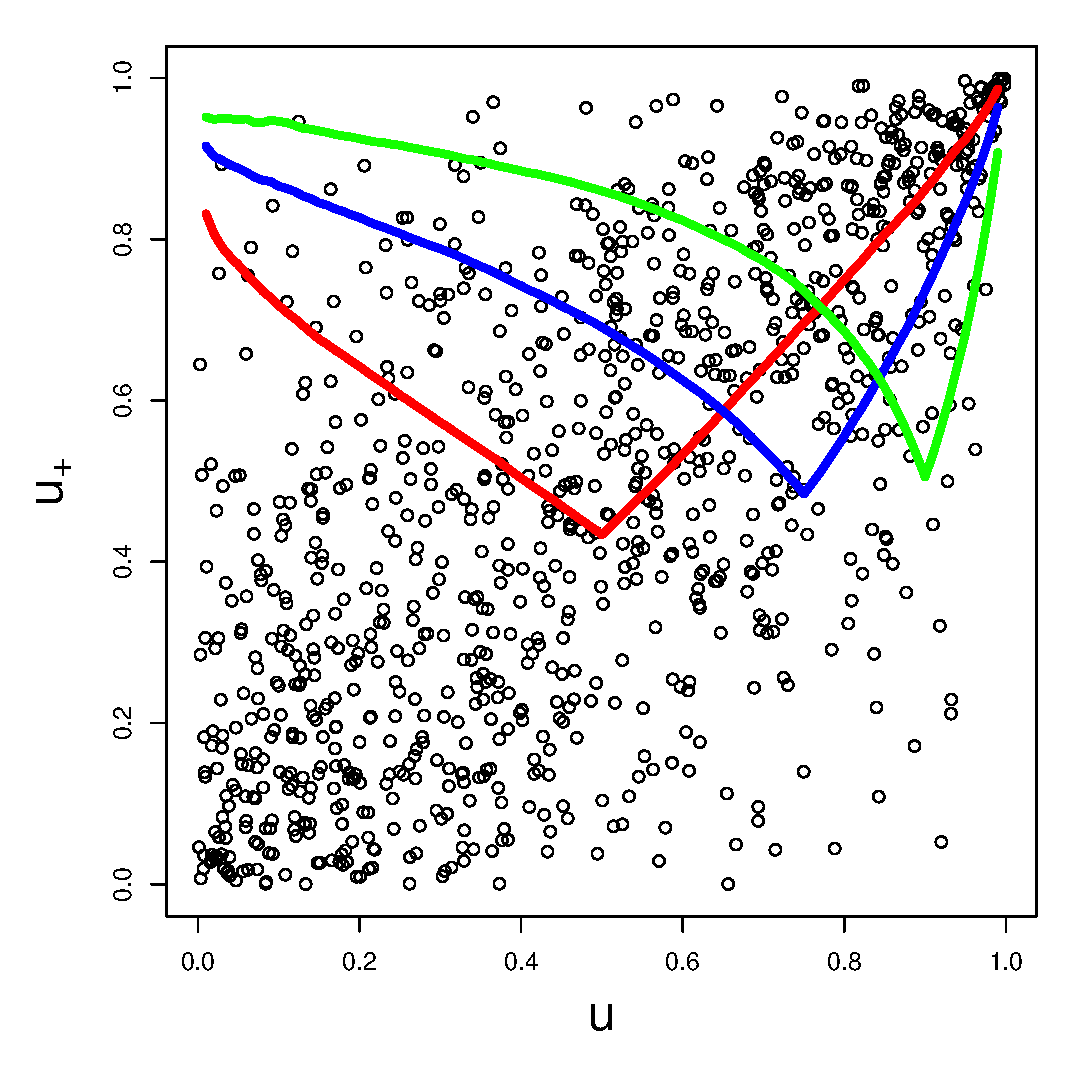
\includegraphics{gumbel.eps}}
      \resizebox{60mm}{!}{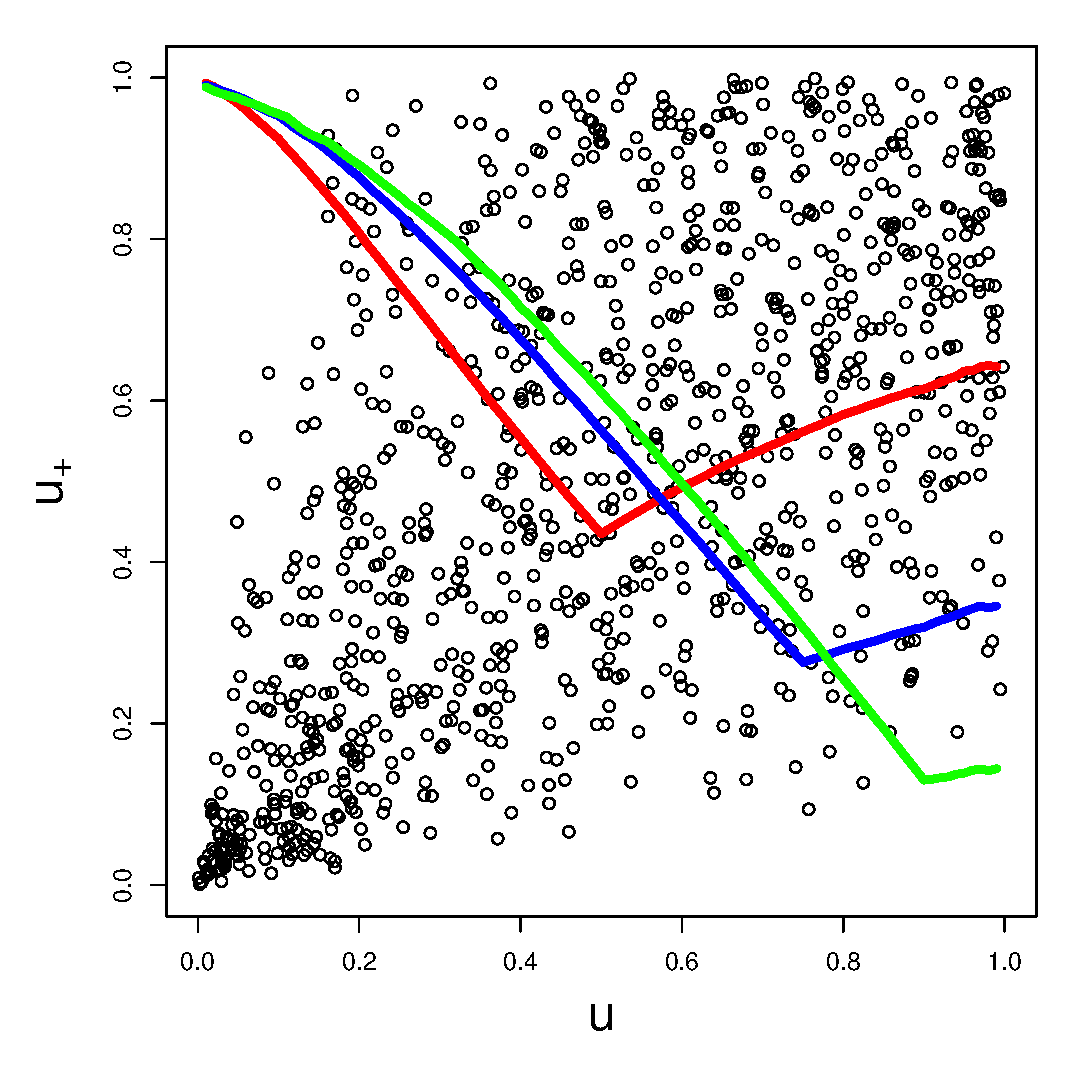
\includegraphics{clayton.eps}}
    \end{tabular}
    \caption{Left and right panels plot $\theta_\alpha$ against $\alpha$ for Gumbel and Clayton copulas respectively. $\theta_\alpha$ is computed assuming a risk aversion function $\phi(u)=(u>t)/(1-t)$ for $t=0.5$ (red), $0.75$ (blue) and $0.9$ (green). The calculation is performed over 100 intervals of $\alpha$ forming $[0,1]$. Note how $\theta_\alpha$ tracks local dependence (clustering along the $45^\circ$ line) in both copulas, apart from the kinks at $\alpha=t$.}
    \label{fsyseg}
  \end{center}
\end{figure}





\section{Sub-aggregate mean and risk densities}\label{ssub}


Write the mean and risk densities of aggregate loss $x_+$ as respectively
$$
m_{\beta,+} = (1-\beta)V_{\beta,+}'
\cq  r_{\beta,+} = \{\beta-\Phi(\beta)\}V_{\beta,+}'
$$
where $V_{\beta,+}$ is the VaR$_\beta$ of $x_+$ and $V_{\beta,+}'$ is the derivative of $V_{\beta,+}$ with respect to $\beta$. Aggregate risk reflects diversification and is therefore composed entirely of systematic risks of component losses forming $x_+$. In addition the VaR$_\beta$--layer of $x_+$ is $I_\beta(u_+)V_{\beta,+}' \de \beta$ where $u_+$ is the percentile rank of $x_+$.

The following allocates aggregate mean and risk densities and aggregate VaR layers to component losses including $x$. The allocation is critical when risk management strategies are applied to layers of $x_+$, and the impact and cost of the strategies are attributed to component losses. Example of such strategies are stop--loss reinsurance and aggregate hedging of a portfolio of losses. The proposed allocation shown below is unbiased and aligns with the overall mean and systematic risk of component losses. The approach relies on conditional mean sharing by \cite{denuit2012convex}.


The aggregate loss is $x_+=\sum_i x_i$ where $x_i$ represents a component loss such as $x$. Using iterated expectations, write $x_+$ as
$$
x_+ = \sum_i g_i(x_+) \cq      g_i(x_+)\equiv \E(x_i|x_+)  \;,
$$
where $g_i$ calculates the mean value of $x_i$ conditional on $x_+$. \cite{denuit2012convex} allocates $g_i(x_+)$ to $x_i$, called conditional mean sharing. The allocation is unbiased since $\E\{g_i(x_+)\}=\E\{\E(x_i|x_+)\}=\E(x_i)$. Substituting $x_+=V_{\beta,+}$ into the above result and taking derivatives with respect to $\beta$ yields
\begin{equation}\label{sharing}
V_{\beta,+}'=  \sum_i \left\{g_i(V_{\beta,+})\right\}'  = V_{\beta,+}' \sum_i g_i'(V_{\beta,+})  \cq \sum_i g_i'(V_{\beta,+})=1\;.
\end{equation}
\eref{sharing} allocates a fraction $g_i'(V_{\beta,+})$ of $V_{\beta,+}'$ to $x_i$, and fractions sum to one across $i$. Apply this fractional allocation to aggregate VaR layers and aggregate mean and risk densities, since all are proportional to $V_{\beta,+}'$. Hence the allocated or ``sub-aggregate" mean and risk densities of $x$ are respectively
$$
\dot{m}_{\beta,+} \equiv m_{\beta,+} g'(V_{\beta,+})
\cq \dot{r}_{\beta,+} \equiv r_{\beta,+} g'(V_{\beta,+}) \;,
$$
where $g(x_+)=\E(x|x_+)$. Identical densities are obtained by performing ground-up calculations on $g(x_+)$ assuming $g$ is increasing and VaR$_\beta$ of $g(x_+)$ is $g(V_{\beta,+})$. Given $\beta$, $\dot{m}_{\beta,+}$ and $\dot{r}_{\beta,+}$ are portions of the mean and risk of VaR$_\beta$--layer of $x_+$ attributable to $x$.



Sub-aggregate mean and risk densities of $x$ are aligned with the overall mean and systematic risk of $x$. Integrating $\dot{m}_{\beta,+}$ over all $\beta$ yields
$$
\int_0^1 \dot{m}_{\beta,+} \de \beta = \int_0^1 (1-\beta) \{g(V_{\beta,+})\}' \de\beta
= \E\{g(x_+)\} = \E(x) \;,
$$
and similarly
$$
\int_0^1 \dot{r}_{\beta,+} \de\beta = \int_0^1 \cov \{I_\beta(u_+),\phi(u_+)\} \{g(V_{\beta,+})\}' \de\beta
$$
$$
=\cov\{g(x_+),\phi(u_+)\}=\cov\{x,\phi(u_+)\}=\overline{r} \;.
$$
Integrating $\dot{m}_{\beta,+}$ and $\dot{r}_{\beta,+}$ over a subset of the unit interval yields an allocation of the mean and risk of the corresponding VaR layer of $x_+$ to $x$.


Sub-aggregate mean and risk densities are different from mean and systematic risk densities: $\dot{m}_{\beta,+} \neq m_\alpha$ and $\dot{r}_\beta \neq \overline{r}_\alpha$ for $\alpha=\beta$, although they integrate to the same result. The former relates to VaR layers of $x_+$ whereas the latter relates to VaR layers of $x$. However equality applies when component losses are comonotonic. This special case is discussed in the next section.



\section{Comonotonicity as a diversification benchmark}\label{scomono}


Comonotonic $x$ and $x_+$ implies $u=u_+$: $x$ and $x_+$ are always at equal percentiles, and $\E(x|x_+)=x$: $x_+$ pinpoints the value of $x$. \cite{dhaene2002concept} and \cite{wang1998comonotonicity} further discuss the concept of comonotonicity. Comonotonicity yields maximum systematic risk across all layers and is hence a benchmark for assessing diversification as shown below.



Comonotonicity between $x$ and $x_+$ implies:
\bi
\i Systematic and standalone risk densities of $x$ are equal, and there is no diversification at any VaR layer of $x$. Since $u=u_+$,
$$
\overline{r}_\alpha = \cov\{I_\alpha(u),\phi(u_+)\}V_\alpha'=\cov\{I_\alpha(u),\phi(u)\}V_\alpha' = r_\alpha \;,
$$
implying $\theta_\alpha=1$. In addition $\overline{r}=r$ and $\theta=1$. This result is discussed in section \aref{sdensity}. Hence $\overline{r}_\alpha$ is maximised across all $\alpha$ under comonotonicity.

\i Sub-aggregate densities are also equal to standalone densities. Since $x=\E(x|x_+)=g(x_+)$, $V_\beta=g(V_{\beta,+})$, hence $V_\beta'=\{g(V_{\beta,+})\}'$ and
$$
\dot{m}_{\beta,+}  = m_\beta \cq \dot{r}_{\beta,+} =r_\beta\;.
$$
Since comonotonic $x_+$ and $x$ reach their VaR$_\beta$--layers simultaneously, the attributed mean and risk of the VaR$_\beta$--layer of $x_+$ to $x$ is the mean and risk (systematic or standalone) of the VaR$_\beta$--layer of $x$.


\ei
The standalone risk density of $x$ thus indicates maximum systematic risk across all layers, and comparing it with systematic and sub-aggregate risk densities of $x$ reveals the extent of diversification in each layer. Section \aref{sdensity} already compares $\overline{r}_\alpha$ with $r_\alpha$ and the ratio characterises the dependence structure of $(x,x_+)$. The following shows a similar interpretation when $\dot{r}_{\beta,+}$ is compared with $r_\beta$. Define the ratio
$$
\gamma_\beta \equiv \frac{\dot{r}_{\beta,+}}{r_\beta} = \frac{\{\beta-\Phi(\beta)\}\{g(V_{\beta,+})\}'}{\{\beta-\Phi(\beta)\}V_\beta'}
=\frac{\{g(V_{\beta,+})\}'}{V_\beta'} =\frac{g'(V_{\beta,+})V_{\beta,+}'}{V_\beta'}
$$
\begin{equation}\label{allratio}
= \frac{\frac{\de}{\de\beta}\E(x|u_+=\beta)}{\frac{\de}{\de\beta}\E(x|u=\beta)}
=\frac{\cov\left\{x,\frac{\de}{\de\beta}\delta_\beta(u_+) \right\}}{\cov\left\{x,\frac{\de}{\de\beta}\delta_\beta(u) \right\}}    \;.
\end{equation}
where $\delta_\beta(u)$ is the Dirac delta function which approaches $\infty$ when $u=\beta$ and is 0 otherwise. Similar to $\theta_\alpha$, $\gamma_\beta=1$ if $u=u_+$ and $\gamma_\beta=0$ if $u$ and $u_+$ are independent. Unlike $\theta_\alpha$, $\gamma_\beta$ is computed entirely from the joint distribution of $(x,x_+)$ and does not involve the risk aversion function $\phi$. In addition $\gamma_\beta$ may exceed one since the numerator in its definition relates to the VaR$_\beta$--layer of $x_+$ whereas the denominator relates to the VaR$_\beta$--layer of $x$ and there is no strict inequality between numerator and denominator.


As per $\theta_\alpha$, $\gamma_\beta$ measures local dependence between $x$ and $x_+$ but in a different manner. The second last expression in \eref{allratio} measures the sensitivity of the conditional expectation of $x$ to changes in $x_+$ at VaR$_\beta$, relative to the same calculation when $u=u_+$. The last expression in \eref{allratio} computes the covariance between $x$ and a function of $u_+$, again relative to the comonotonic case.



\fref{fsyseg2} plots $\gamma_\beta$ against $\beta$ using copulas in \fref{fsyseg}. Assume exponential and normal distributions for $x$. Note $\gamma_\beta$ is independent of location and scale of $x$. Calculations show $\gamma_\beta>1$ over some values of $\beta$ hence $\gamma_\beta$ is scaled by its maximum value over $\beta$ so that resulting values do not exceed $1$. Similar to $\theta_\alpha$,  $\gamma_\beta$ traces the local dependence structure of $(x,x_+)$: the dispersion between scatter points along the 45$^\circ$ line. However calculated values of  $\gamma_\beta$ are more volatile than $\theta_\alpha$ as the former involve conditional expectations over narrow windows whereas the latter use conditional tail expectations.

\begin{figure}
  \begin{center}
    \begin{tabular}{cc}
      \resizebox{60mm}{!}{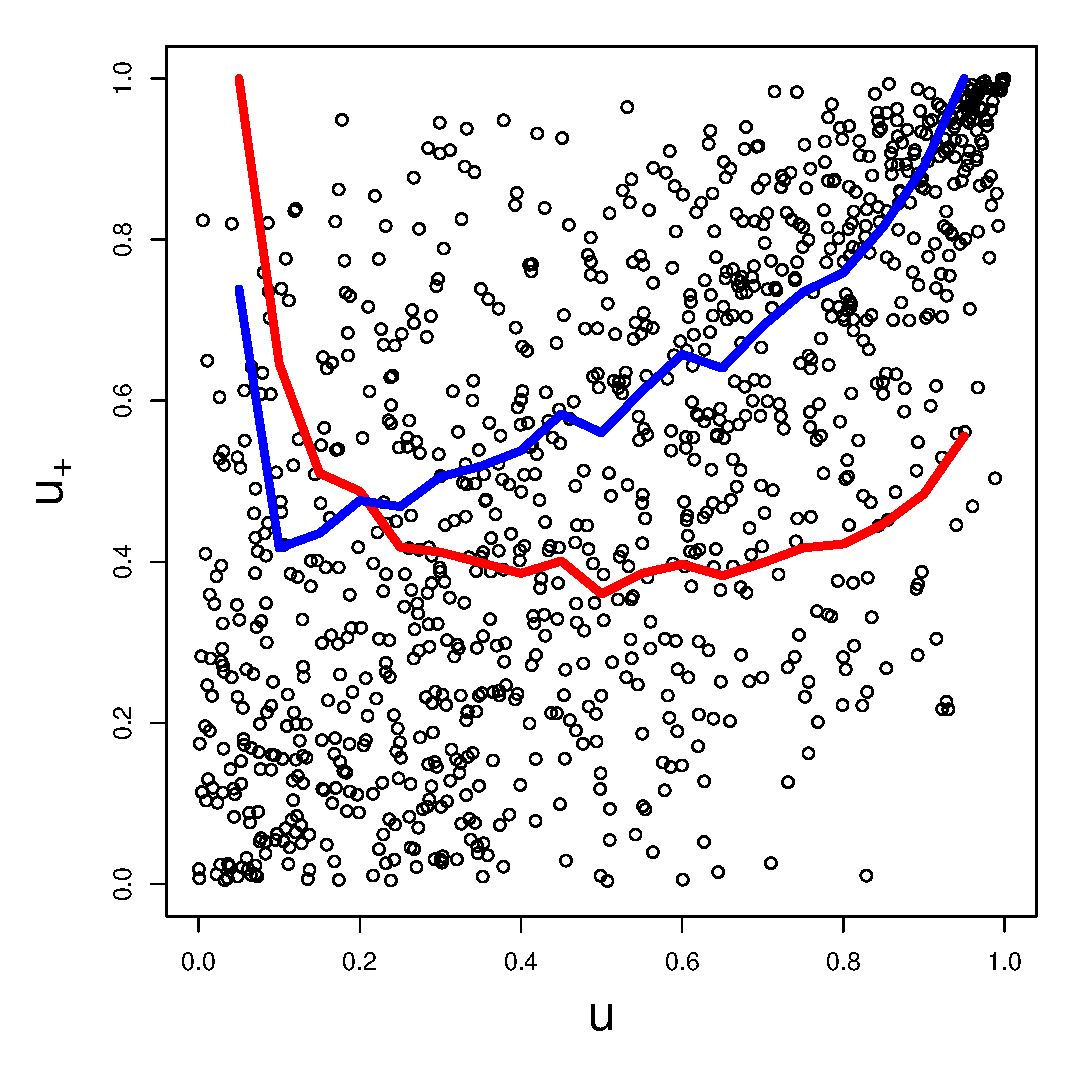
\includegraphics{gumbelnew.eps}}
      \resizebox{60mm}{!}{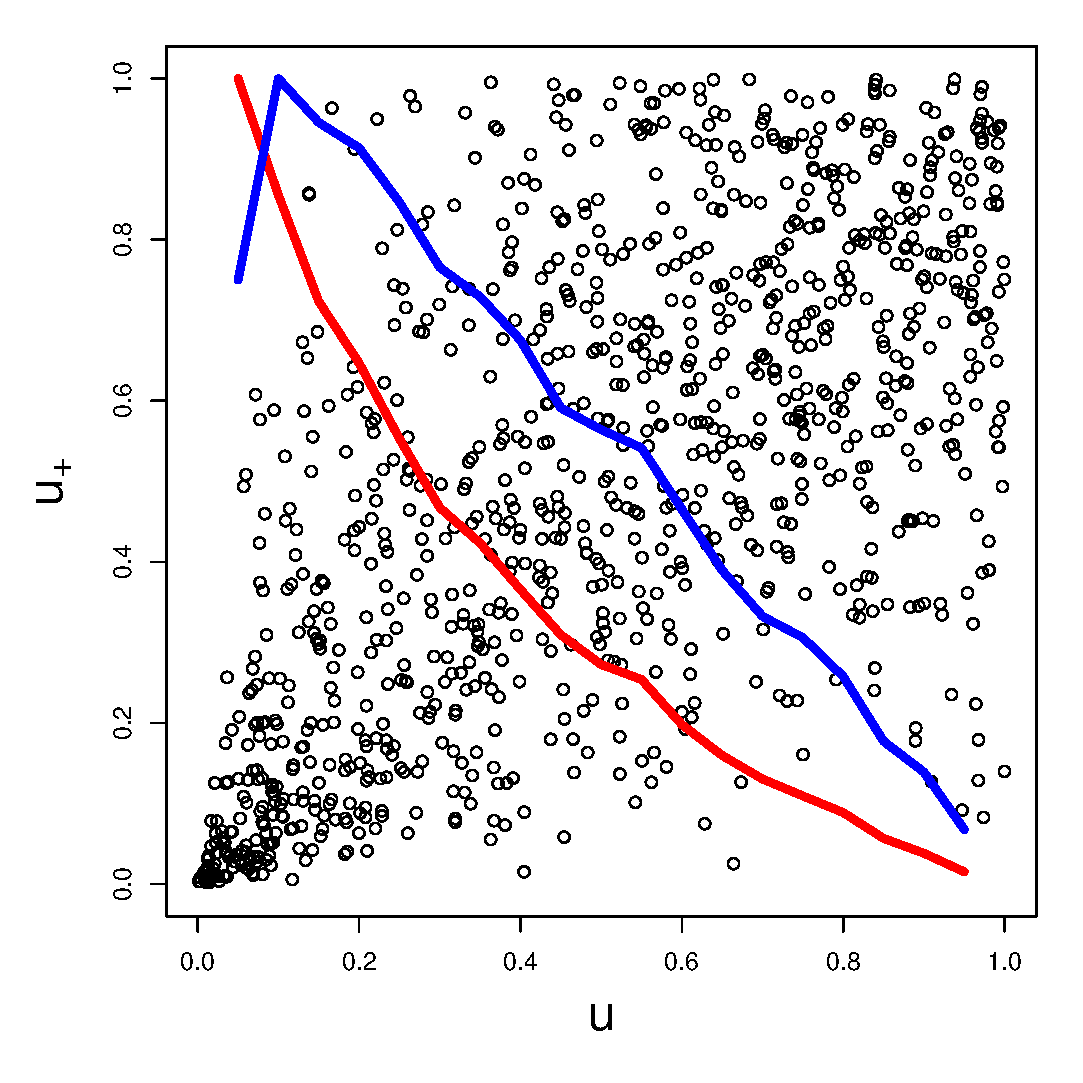
\includegraphics{claytonnew.eps}}
    \end{tabular}
    \caption{Left and right panels plot $\gamma_\beta/\max_\beta(\gamma_\beta)$ against $\beta$ for Gumbel and Clayton copulas respectively. $\gamma_\beta$ is computed assuming $x$ is exponential (red) and normal (blue). The calculation is performed over 20 intervals of $\beta$ forming $[0,1]$ to produce smoother curves. Note how the curves trace the dependence structure of $(u,u_+)$ represented by the scatter of points along the 45$^\circ$ line.}
    \label{fsyseg2}
  \end{center}
\end{figure}




\section{Case study using historical stock returns}\label{seg}

This section applies the proposed systematic risk and diversification analytical framework to daily NASDAQ, S\&P and FTSE returns between 1985 and 2015. Form a hypothetical portfolio of \$100 in each market index, and assume the empirical joint probability distribution. To be consistent with the proposed framework, focus on investment losses rather than gains. Hence switch the signs of investment returns, with gains being negative losses. Use the risk aversion function $\phi(\alpha)=4I_{0.75}(\alpha)$, hence risk is the mean loss above VaR$_{0.75}$ compared to the overall mean.

Top four panels in \fref{fcase1} display empirical marginal probability distributions and copulas of hypothetical index losses. NASDAQ lossess are the most skewed, while S\&P losses are the most peaked. In addition NASDAQ and S\&P losses are highly dependent, and both are less dependent overall on FTSE losses (presumably due to different geographical location). All three market indices exhibit significant upper and lower tail dependence: extreme losses and gains are highly dependent across markets.

Bottom two panels in \fref{fcase1} graph standalone and systematic risk densities for each market index, calculated from the empirical joint probability distribution. Density values are smoothed to reduce volatility across VaR layers. Before aggregation, NASDAQ has the highest risk density due to greater skewness of its probability distribution. S\&P and FTSE have similar risk densities, although S\&P has a slightly lower density in middle VaR layers due to greater peakedness of its probability density. All three risk densities are reduced after diversification, most notably FTSE. Subsequent figures compare and analyse standalone and systematic risk densities.


\fref{fcase2} compares standalone and systematic risk densities for each market index. Systematic risk ratios, and copulas between index and aggregate losses, are also shown. Note from \sref{sdensity} that systematic risk ratios are computed entirely from the copulas and summarise the dependence structure. Also note the kink in systematic risk ratios at VaR$_{0.75}$--layers due to the selection of the risk aversion function. FTSE has lower systematic risk ratios than NASDAQ and S\&P across all VaR layers due to its weaker dependence with the aggregate loss. Hence FTSE experiences stronger diversification. All three market indices have systematic risk ratios close to 1 in extreme VaR layers, due to tail dependence. Therefore there is minimal risk diversification in extreme VaR layers of all three indices.

Table 1 shows overall risks for each market index, before and after diversification. Overall systematic risk ratios are also shown. As expected NASDAQ has the highest standalone and systematic risk. S\&P and FTSE have similar standalone risks, although FTSE has higher diversification and therefore lower systematic risk. NASDAQ and S\&P have similar overall systematic risk ratios.

\begin{table}[h]
  \begin{center}
\begin{tabular}{l|c|c|c }

 Portfolio & $r$ & $\overline{r}$ & $\theta$ \\
 \hline
 NASDAQ & \$2.00 & \$1.86 & 0.93\\
 S\&P & \$1.32 & \$1.22 & 0.92\\
 FTSE & \$1.31 & \$0.87 & 0.66\\

  Overall & \$4.63 & \$3.95 & 0.85 \\
 \hline
\end{tabular}
\caption{Overall standalone risk, systematic risk and risk ratio for each market index.}
  \end{center}
\end{table}




\fref{fcase3} shows mean and risk densities of the aggregate portfolio loss and its breakdown into sub-aggregate densities. NASDAQ generally has a higher sub-aggregate mean and risk density, notably in high VaR layers of the aggregate loss, due to its higher skewness and systematic risk contribution. Note from \sref{ssub} that sub-aggregate mean and risk densities integrate to the overall mean and systematic risk of each market index.


\begin{figure}
  \begin{center}
    \begin{tabular}{cc}
      \resizebox{60mm}{!}{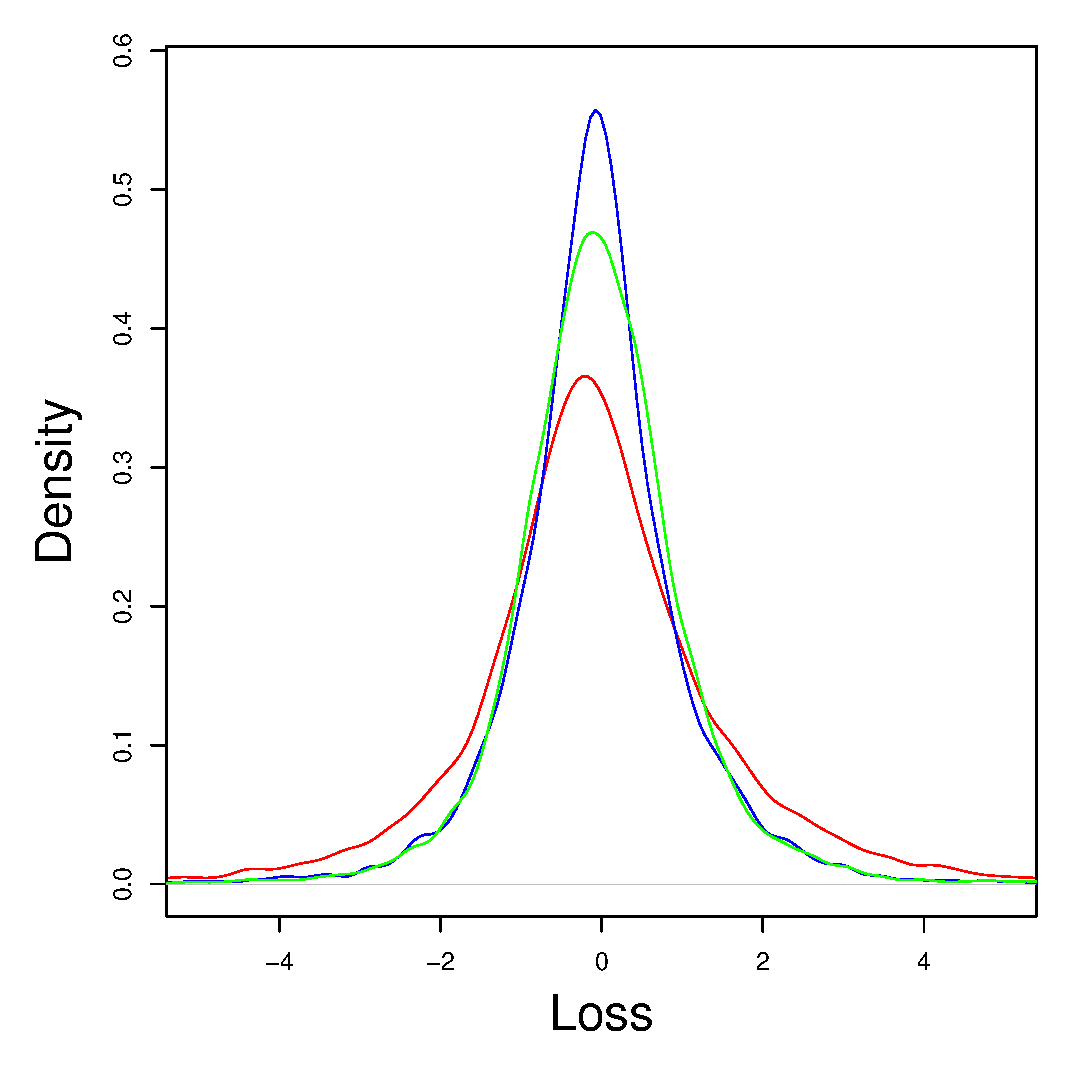
\includegraphics{density.eps}}
      \resizebox{60mm}{!}{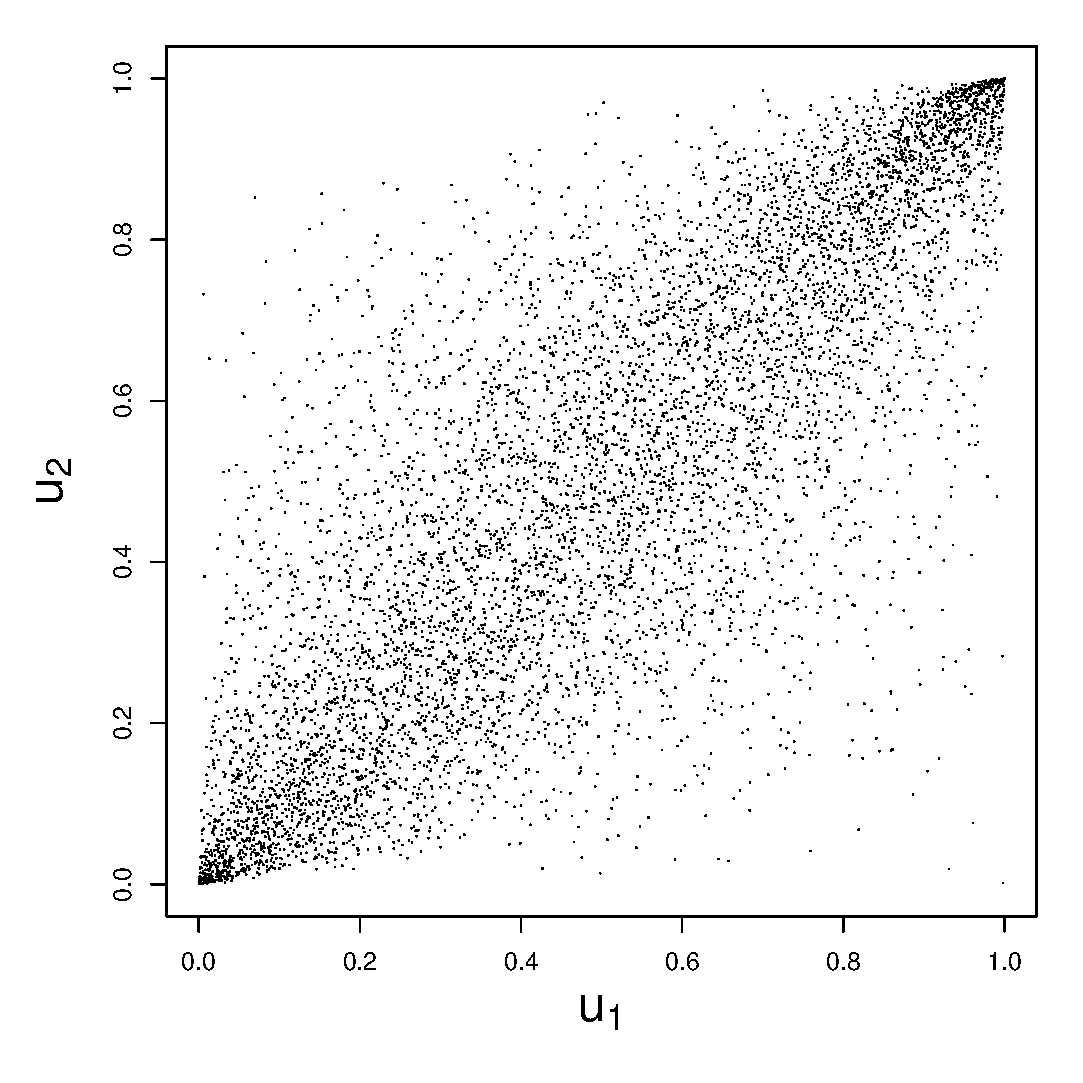
\includegraphics{nasdaqsp.eps}}\\
      \resizebox{60mm}{!}{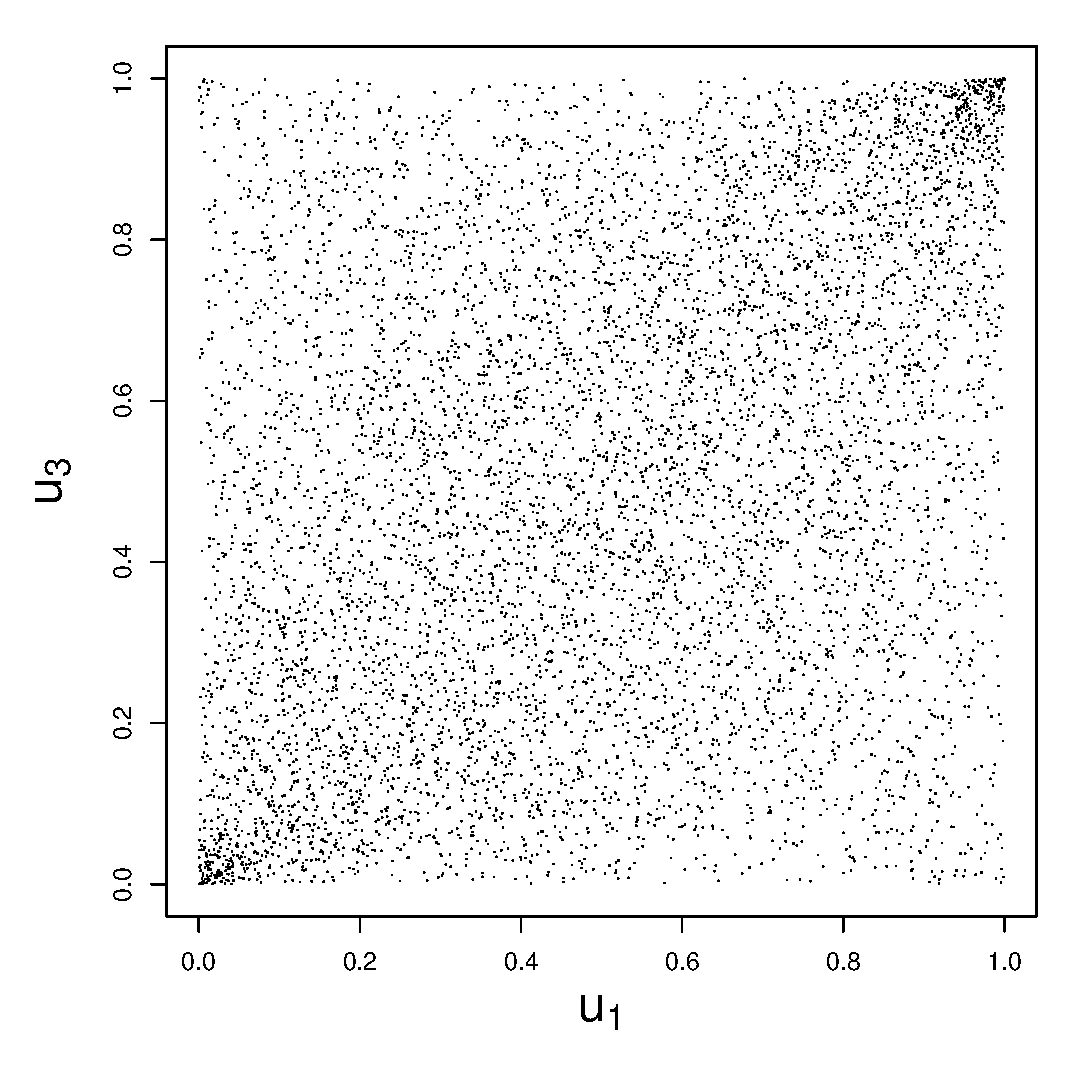
\includegraphics{nasdaqftse.eps}}
      \resizebox{60mm}{!}{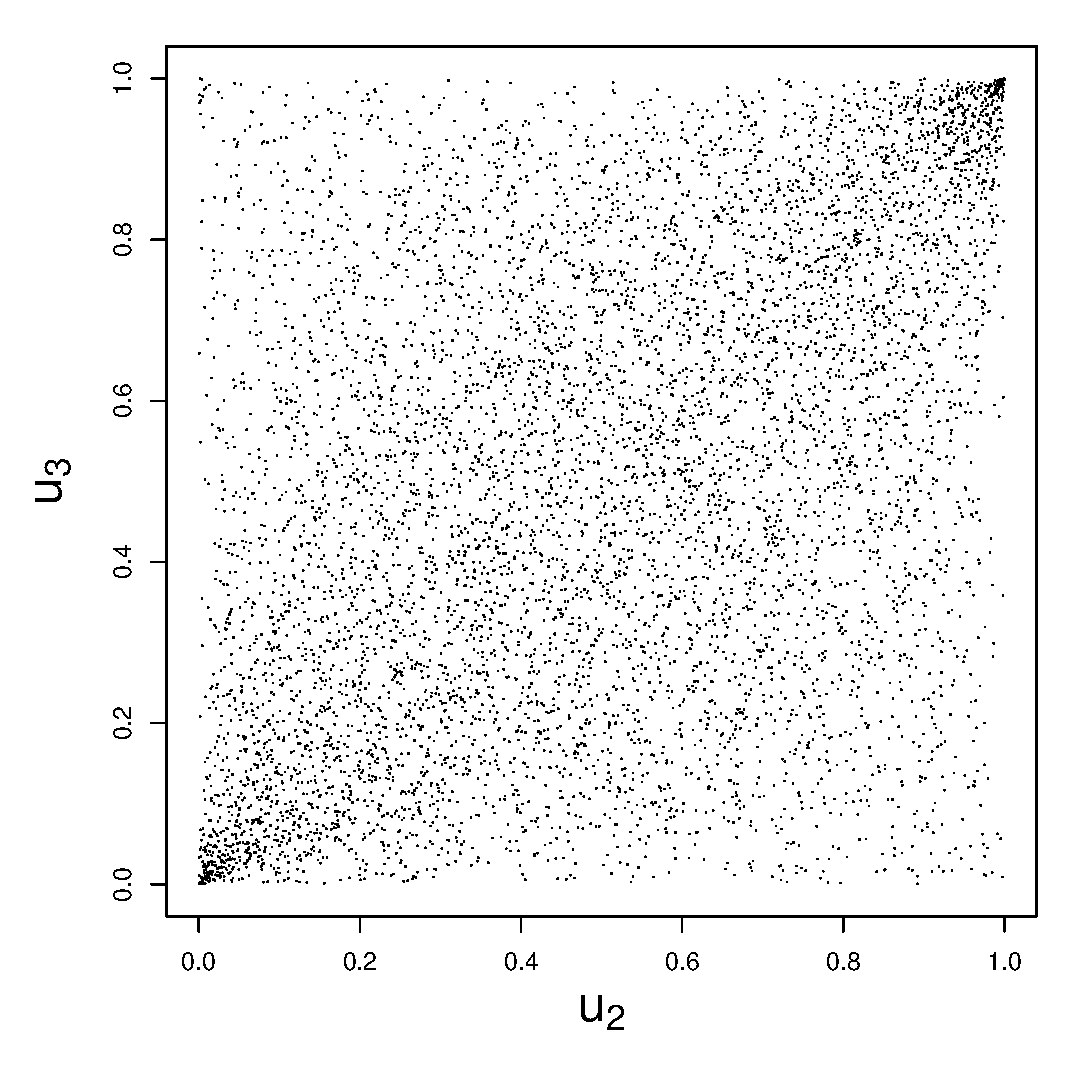
\includegraphics{spftse.eps}}\\
       \resizebox{60mm}{!}{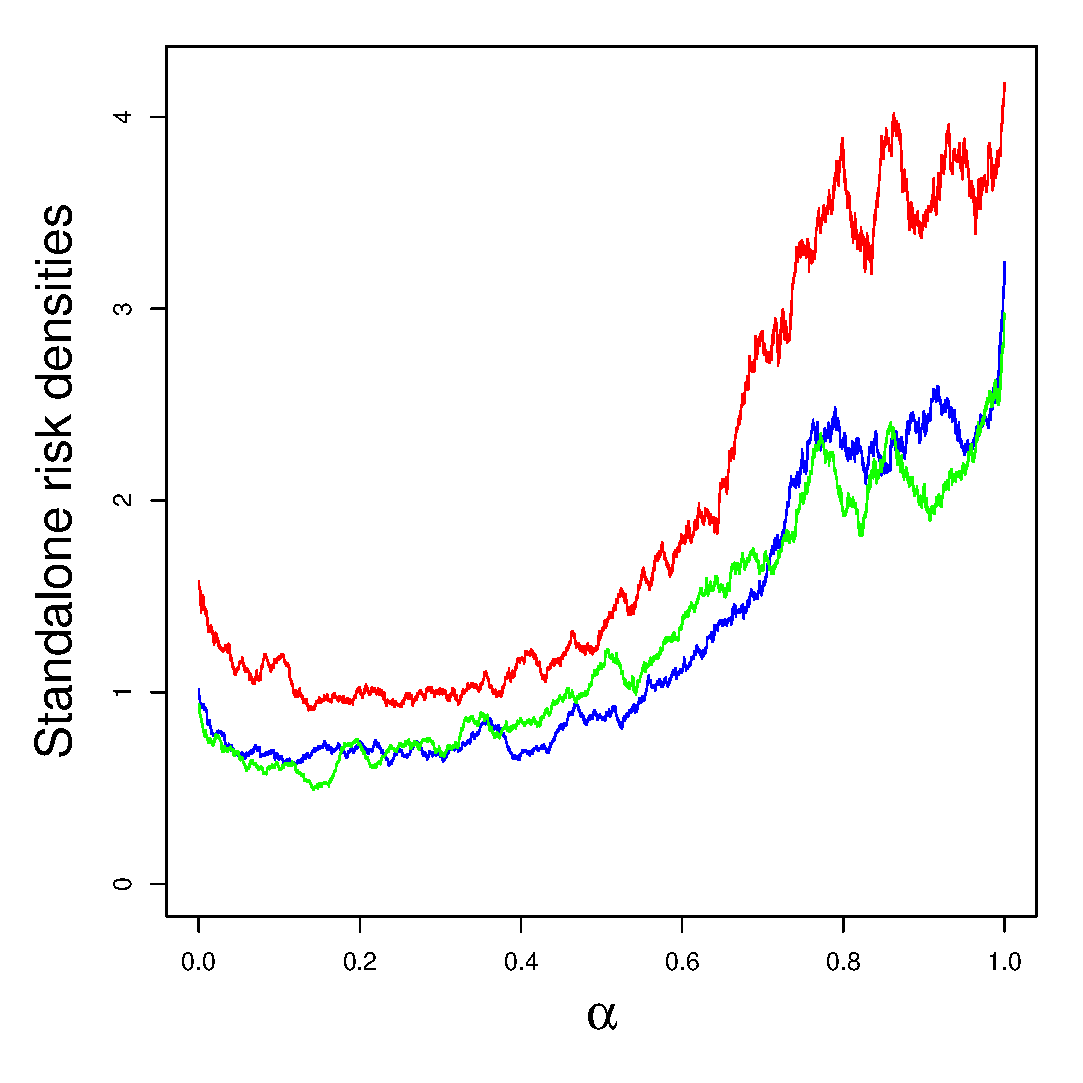
\includegraphics{risk1.eps}}
      \resizebox{60mm}{!}{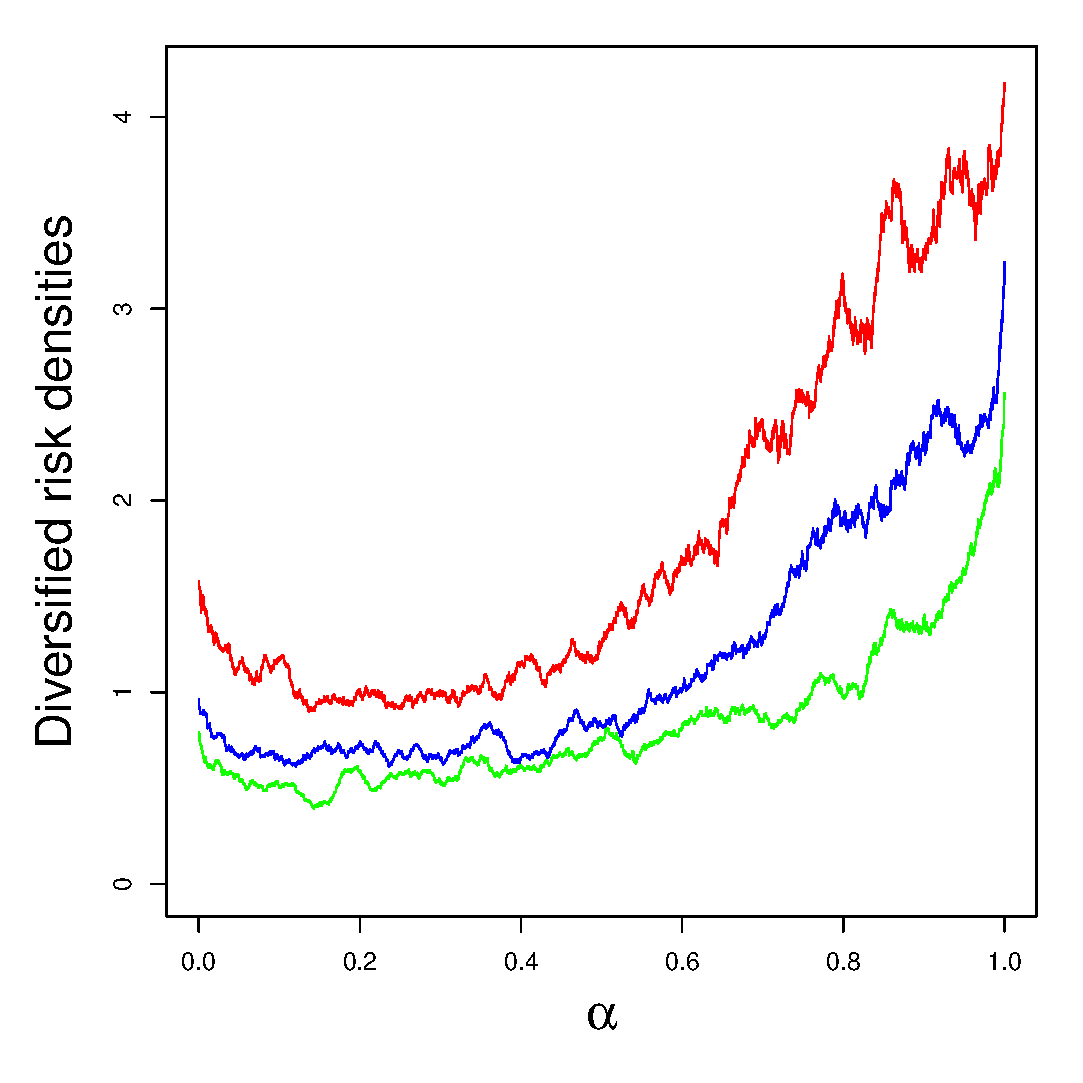
\includegraphics{risk2.eps}}\\
    \end{tabular}
    \caption{Top left panel plots empirical probability densities. Next 3 top panels plot empirical copulas ($u_1$:NASDAQ, $u_2$: S\&P, $u_3$: FTSE). Bottom left and right panels plot calculated standalone and systematic risk densities, respectively. Red, blue and green represent NASDAQ, S\&P and FTSE, respectively.}
    \label{fcase1}
  \end{center}
\end{figure}


\begin{figure}
  \begin{center}
    \begin{tabular}{cc}
      \resizebox{60mm}{!}{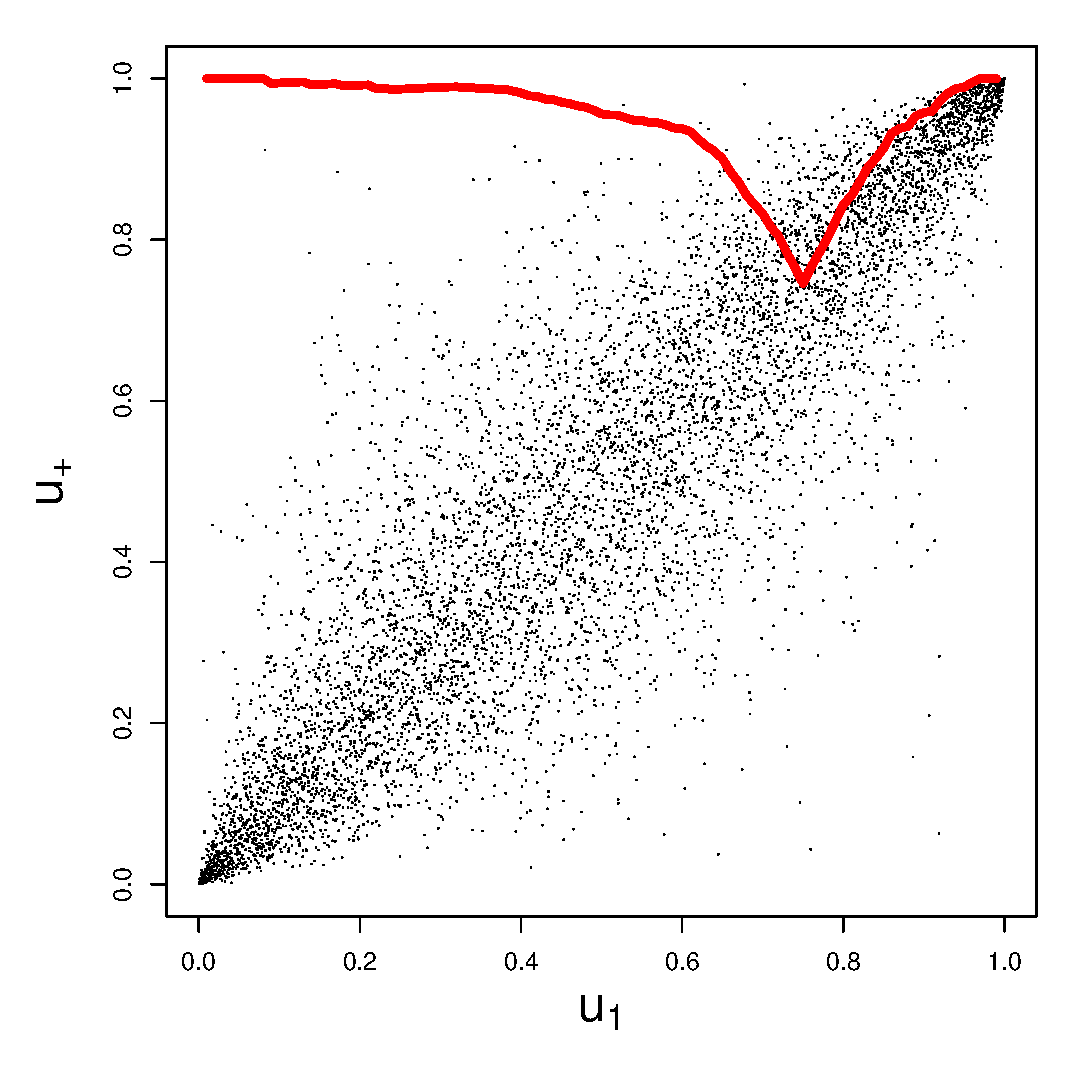
\includegraphics{nasdaqcop.eps}}
      \resizebox{60mm}{!}{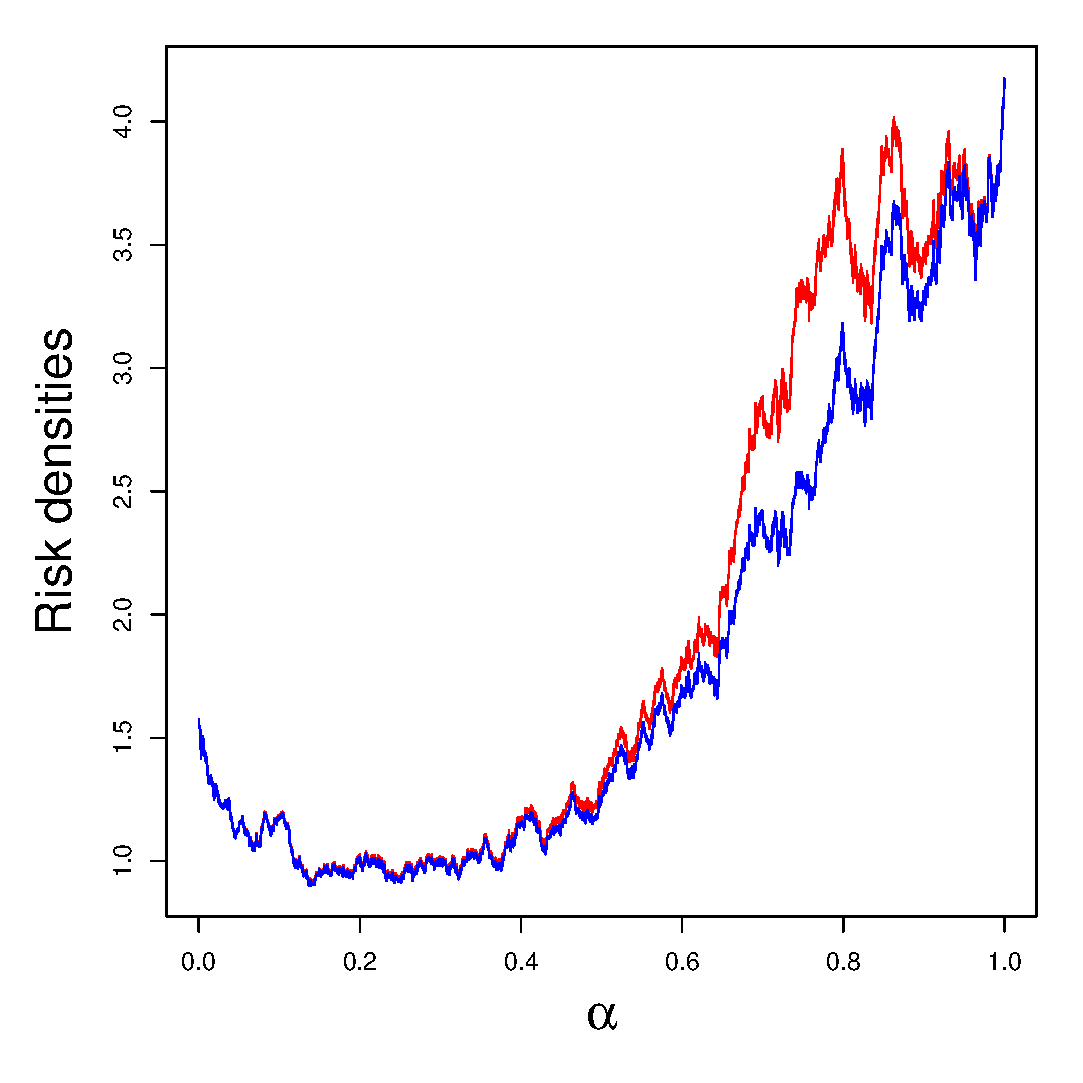
\includegraphics{nasdaqrisk.eps}}\\
      \resizebox{60mm}{!}{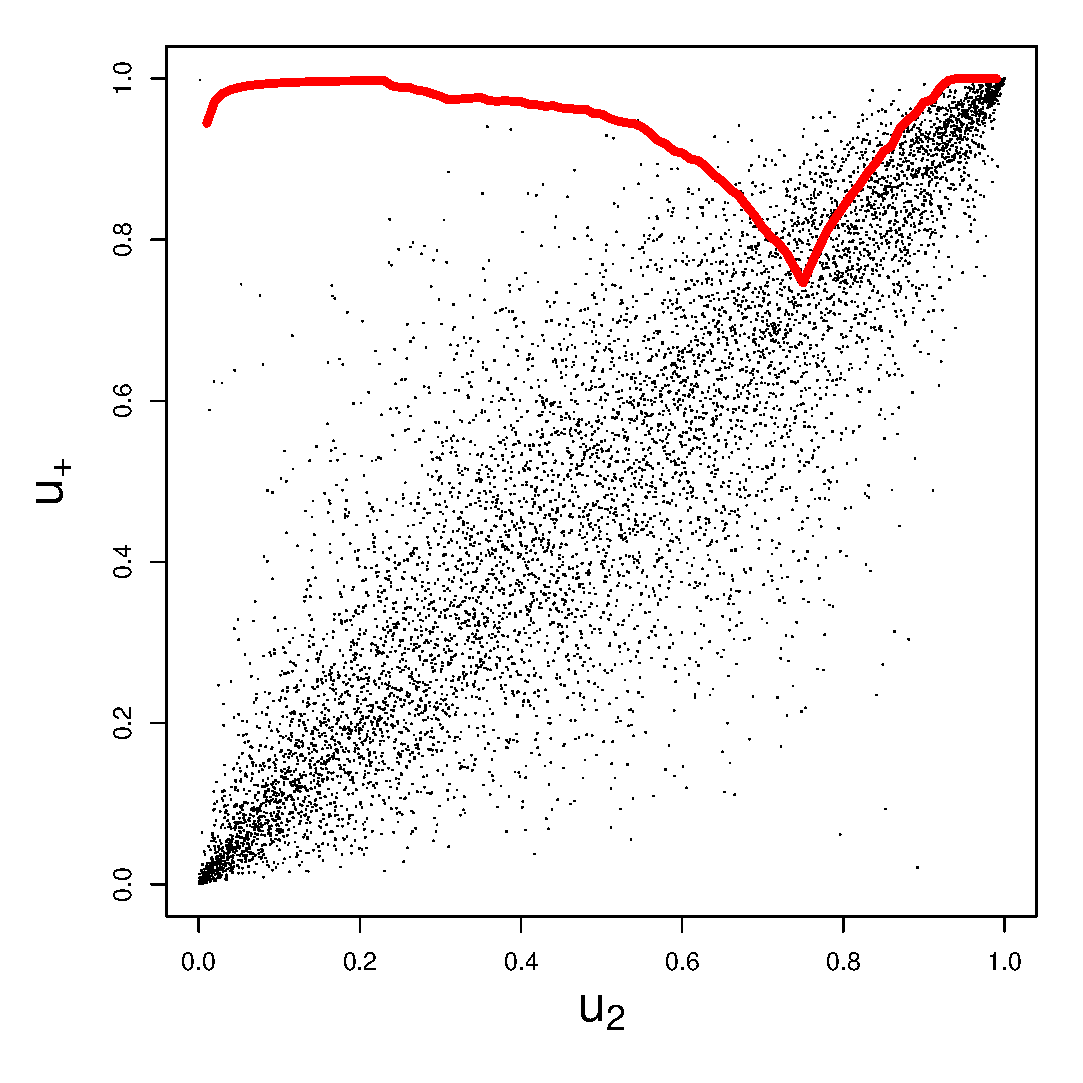
\includegraphics{spcop.eps}}
      \resizebox{60mm}{!}{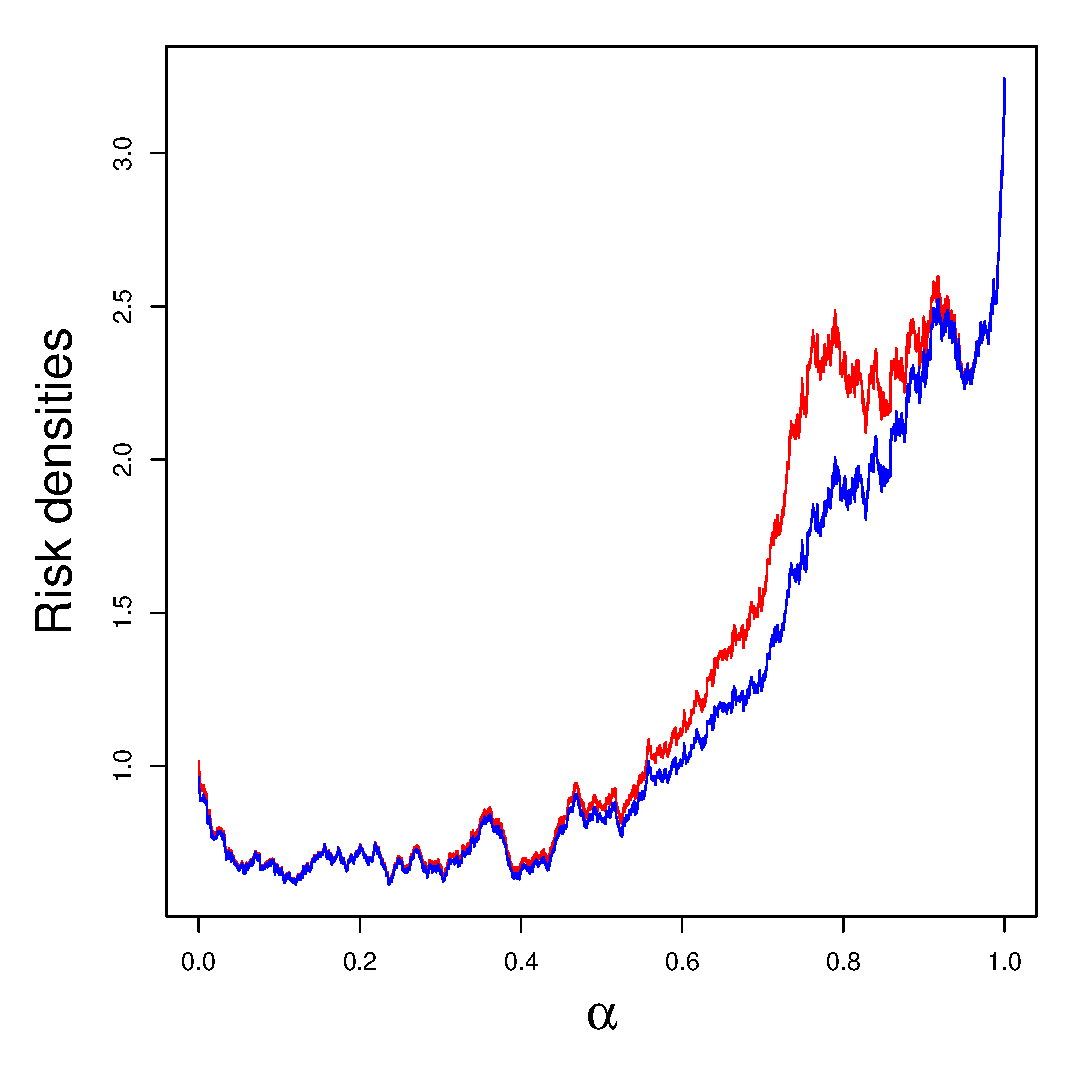
\includegraphics{sprisk.eps}}\\
      \resizebox{60mm}{!}{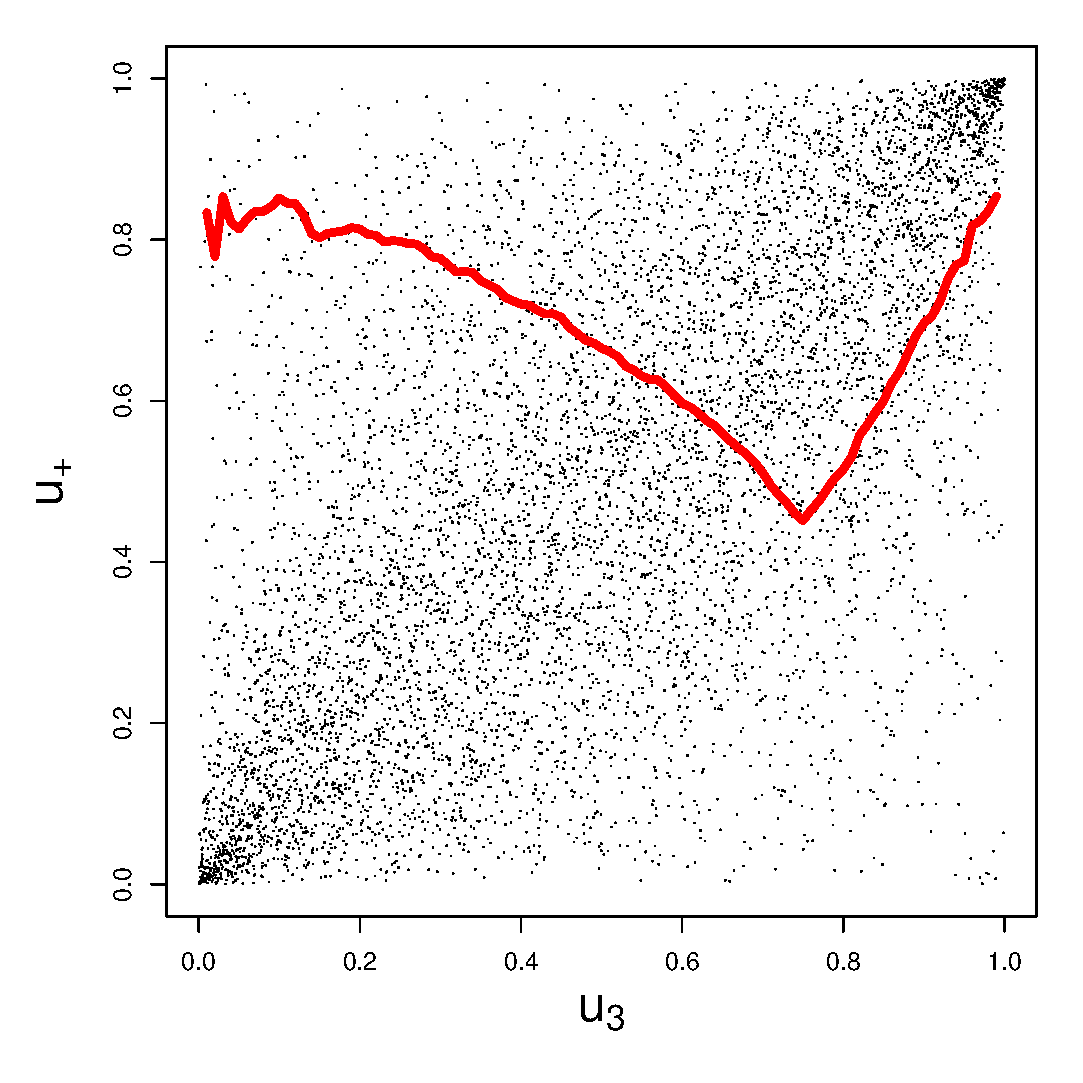
\includegraphics{ftsecop.eps}}
      \resizebox{60mm}{!}{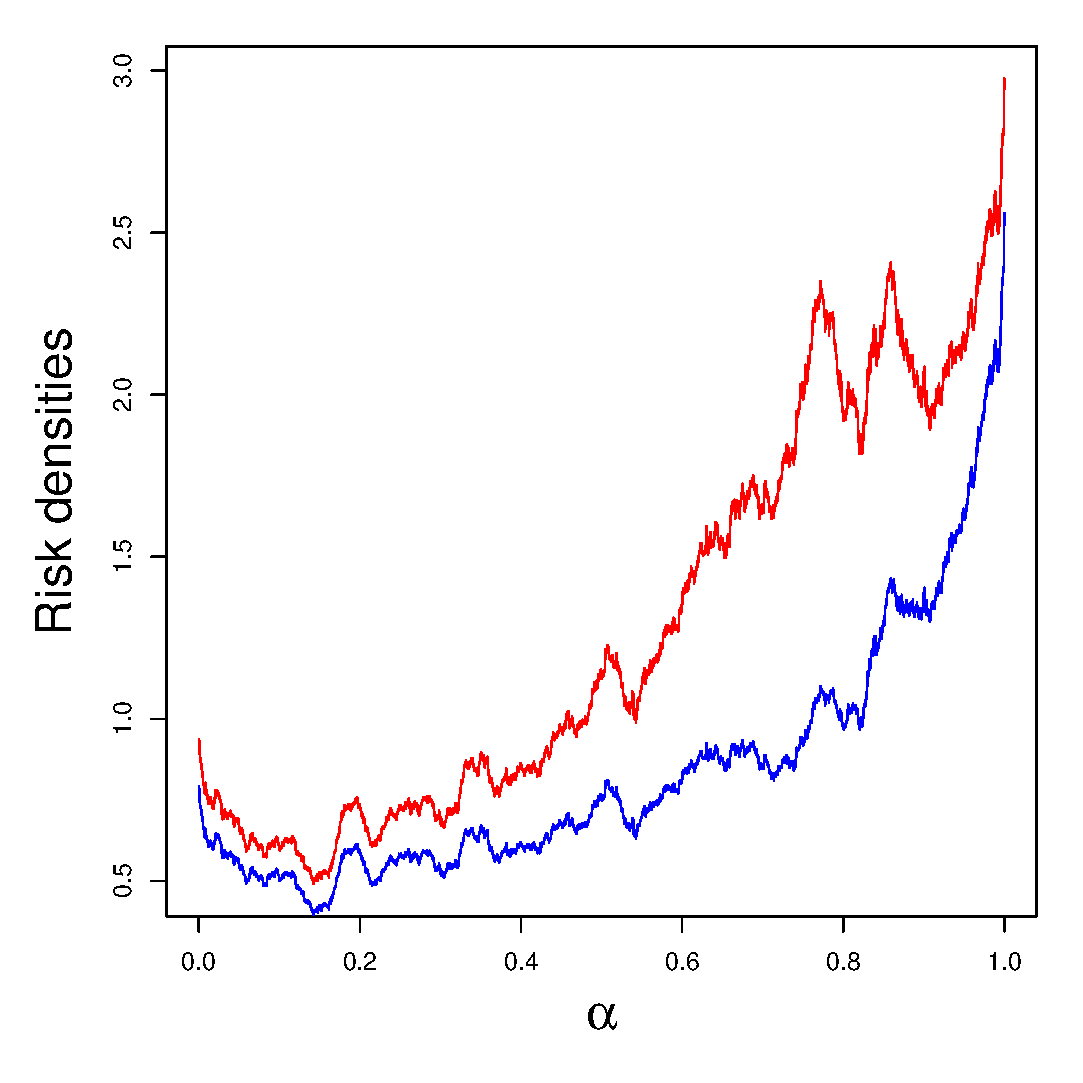
\includegraphics{ftserisk.eps}}\\
    \end{tabular}
    \caption{Left panels plot historical $(u_i,u_+)$ and, in red, $(\alpha,\theta_\alpha)$. Right panels plot calculated $(\alpha,r_\alpha)$ in red and $(\alpha,\overline{r}_\alpha)$ in blue. Note $\theta_\alpha=\overline{r}_\alpha/r_\alpha$. Top, middle and bottom panels are for NASDAQ, S\&P and FTSE, respectively.}
    \label{fcase2}
  \end{center}
\end{figure}


\begin{figure}
  \begin{center}
    \begin{tabular}{cc}
      \resizebox{60mm}{!}{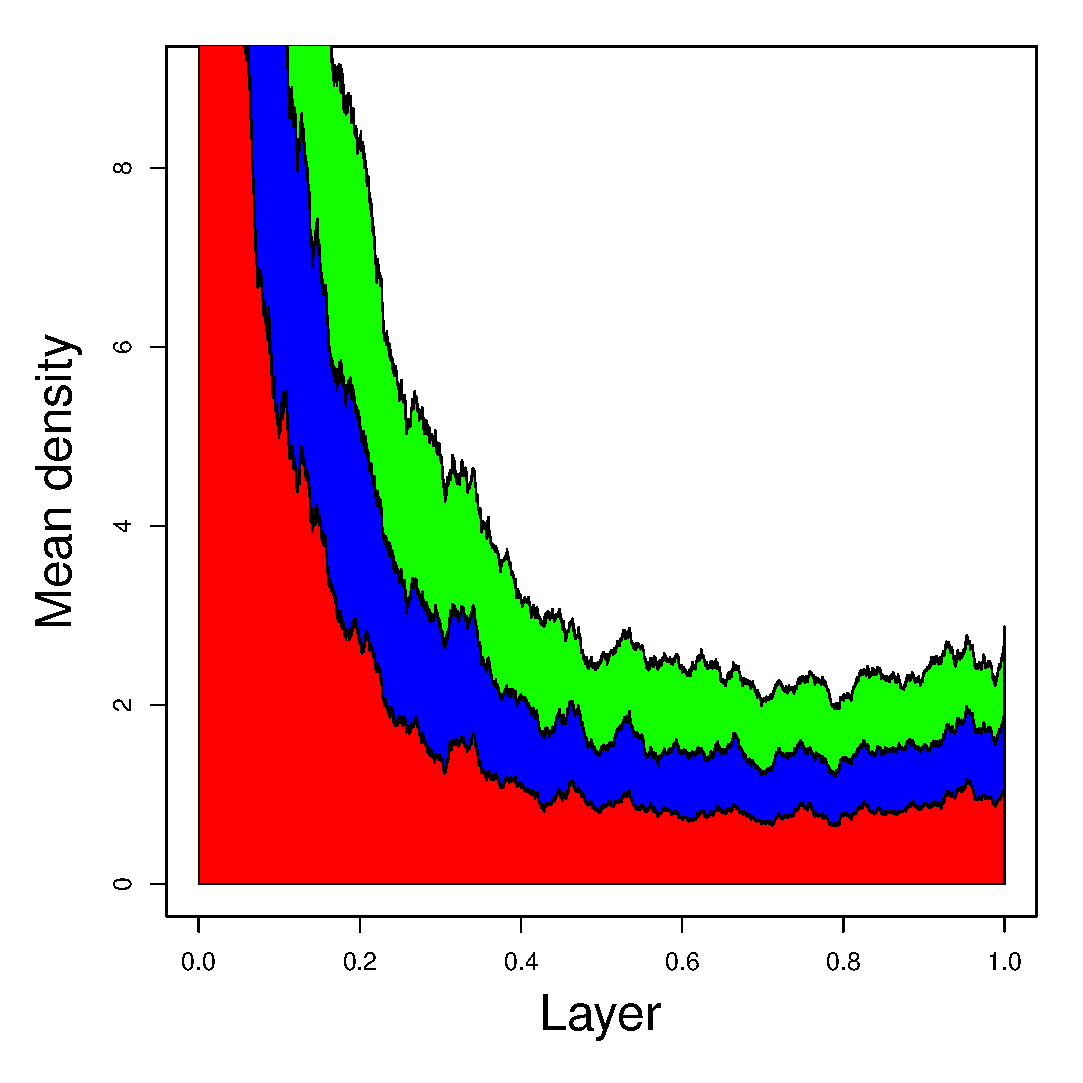
\includegraphics{aggmean.eps}}
      \resizebox{60mm}{!}{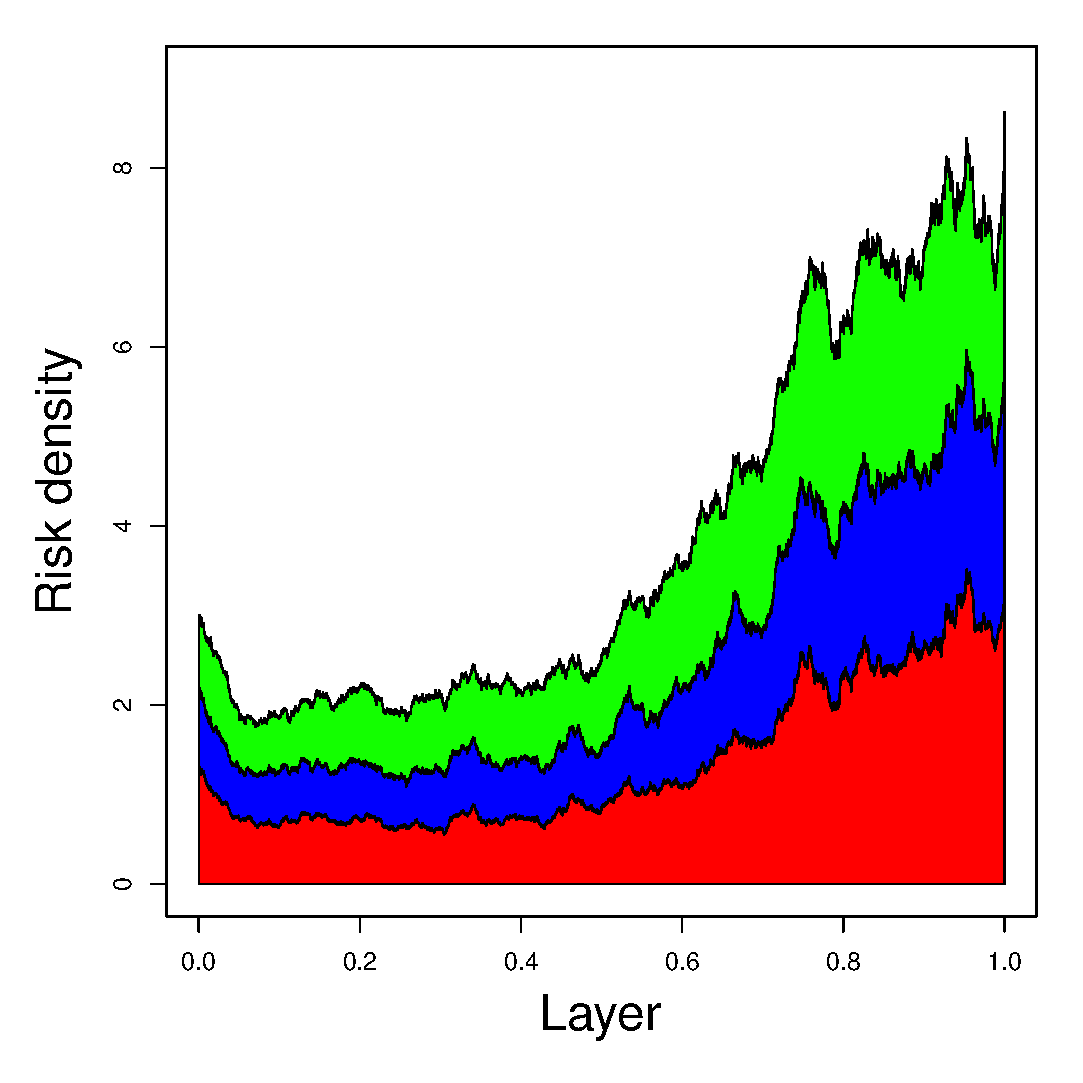
\includegraphics{aggrisk.eps}}\\
    \end{tabular}
    \caption{Left panel shows aggregate mean density and its breakdown into sub-aggregate mean densities. Right panel shows the same, for risk densities. Red, blue and green represent NASDAQ, S\&P and FTSE, respectively.}
    \label{fcase3}
  \end{center}
\end{figure}




Figures \aref{fcase1}, \aref{fcase2} and \aref{fcase3} guide the formulation of effective risk management strategies. For example standalone and systematic risks are concentrated in high VaR layers and can be significantly reduced with put options. In addition, from \fref{fcase2}, dependence is strong at high VaR layers and weaker at lower VaR layers, hence diversification is improved when high VaR layers are eliminated. Consider two scenarios: put options on each market index and an aggregate put option on the portfolio. Assume an exercise price of VaR$_{0.95}$ of the loss referenced in the put option. Risks after put options  are areas under risk densities up to the exercise price. Summary results of the first scenario are shown in table 2 in a similar format as table 1. Under the second scenario, aggregate risk after diversification is $3.55$ hence the first scenario is more risk-effective without considering option prices.

\begin{table}[h]
  \begin{center}
\begin{tabular}{l|c|c|c }

 Portfolio & $r$ & $\overline{r}$ & $\theta$ \\
 \hline
 NASDAQ & \$1.81 & \$1.67 & 0.92\\
 S\&P & \$1.17 & \$1.07 & 0.91\\
 FTSE & \$1.17 & \$0.75 & 0.64\\
 Overall & \$4.15 & \$3.49 & 0.84 \\
 \hline
\end{tabular}
\caption{Overall standalone risk, systematic risk and risk ratio for each market index, after purchasing put options at exercise price $V_{0.95}$ for each index. }
  \end{center}
\end{table}




\newpage

\section*{References}


\bibliography{PhD}



\end{document}
